Recently, an interdisciplinary research between the fields of Computer Science and Biology has been rapidly growing. Natural computing consists of three classes of methods:
\begin{itemize}
  \item those that are based on the use of computers to synthesize natural phenomena
  \item those that employ natural materials (e.g., molecules) to compute
  \item those that take inspiration from nature for the development of novel problem-solving techniques
\end{itemize}

% Bioinformatics (slaves of biologists)

\section{Bioinformatics} % (fold)
\label{sec:bioinformatics}

Bioinformatics has undergone a fast evolving process, especially the areas of genomics and proteomics. Bioinformatics can be seen as the application of computing tools and techniques for the management of biological data. Just to mention a few:
\begin{itemize} 
  \item the design of efficient algorithms for DNA sequence alignment,
  \item the investigation of methods for prediction of the 3D structure of molecules and proteins,
  \item the development of data structures to effectively store huge amount of structured data.
\end{itemize}

% section bioinformatics (end)

\section{Biomolecular computing} % (fold)
\label{sec:biomolecular_computing}

Biomolecular computing make use of molecules such as DNA and proteins to perform computations involving storing, retrieving and processing data. It takes advantage of the many different molecules to try many different possibilities at one, so it is somewhat similar to parallel computing.

Adleman in his 1994 report \cite{Adleman1994MolecularComputation} demonstrated a proof of concept use of DNA as a form of computation which solved the Hamiltonian path problem. Since then, various Turing machines have been proven to be constructible with DNA \cite{Kari2000DNAPCP}. 

DNA can also be used as a digital data storage with 5.5 petabits per cubic millimeter of DNA (see \cite{Church2012DNAStorage}). The information retrieval is, however, a slow process, as the DNA needs to be sequenced in order to retrieve data, so this method is intended mainly for a long-term archival of large amounts of scientific data.

% section biomolecular_computing (end)

\section{Biologically inspired computing models} % (fold)
\label{sec:biologically_inspired_computing_models}


On the other hand, the birth of biologically inspired frameworks started the investigation of mathematical models and their properties and technological requirements for their implementation by biological hardware.
Those frameworks are inspired by the nature in the way it ``computes'', and has gone through the evolution for billions of years.

Neural networks, genetic algorithms and DNA computing are already well established research fields.

\subsection{Neural networks} % (fold)
\label{sub:neural_networks}

Inspired by the human brain, which contains on average 86 billions neurons \cite{Azevedo09NumberOfNeurons}, neurophysiologist Warren McCulloch in 1943 proposed a mathematical model of artificial neural network.

A single perceptron computes a function $f(x)$, where $x$ is an input - a vector of real values.

The perceptron can learn itself by modifying parameters used to compute the function. This learning can be performed in various ways, we will mention only the supervised learning. Imagine a function with
\begin{itemize}
  \item input: perceptron's parameters
  \item output: error of the computed result $f(x)$
\end{itemize}
If the perceptron receives a feedback in form of error (from the supervision, e.g. dataset used to train the perceptron), it can modify it's parameters such the error will be minimized in the future. This can be done through the gradient descent method, which is used to find a local minimum of a function.

A single perceptron can only compute linear functions, so they are often connected with other perceptron to form a neural network. Often it is practically unusable to say what is the purpose of a single neuron in a more complex neural networks.

Neural networks have broad applicability to real world problems and are best if the modeled system has some tolerance to error such as:
\begin{itemize}
  \item Image recognition: OCR, web search by image
  \item Music recognition by voice sample
  \item Time series forecast: weather, stock
  \item Diagnosing of illnesses
\end{itemize}

% subsection neural_networks (end)

\subsection{Evolutionary algorithms} % (fold)
\label{sub:evolutionary_algorithms}

Evolutionary algorithms are inspired by Darwin's theory of evolution. Basically, an algorithm starts with a population of random individuals (solutions to the problem). In each generation, the fitness of every individual is evaluated and the more fit individuals are replicated and mutated to form a new population. The less fit individuals die.

Idea of evolutionary computing was introduced in the 1960's by I. Rechenberg. Nowadays they have been applied to find solution of many optimization problems. They also can be used to design or to train a neural network \cite{Montana:1989:TrainNeuronByGenetic}.

% subsection evolutionary_algorithms (end)

% Membranes

\subsection{Membrane systems} % (fold)
\label{sub:membrane_systems}

However, nature computes not only at the neural or genetic level, but also at the cellular level. In general, any non-trivial biological system has a hierarchical structure where objects and information flows between regions, what can be interpreted as a computation process.

The regions are typically delimited by various types of membranes at different levels from cell membranes, through skin membrane to virtual membranes which delimits different parts of an ecosystem.
This hierarchical system can be seen in other field such as distributed computing, where again well delimited computing units coexist and are hierarchically arranged in complex systems from single processors to the internet.

Membranes keep together certain chemicals or information and selectively determines which of them may pass through.

% The notion of membrane structure

From these observations, P\u{a}un \cite{Paun98} introduces the notion of a membrane structure as a mathematical representation of hierarchical architectures composed of membranes. It is usually represented as a Venn diagram with all the considered sets being subsets of a unique set and not allowed to be intersected. Every two sets are either one the subset of the other, or disjoint. Outermost membrane (also called skin membrane) delimits the finite ``inside'' and the infinite ``outside''.

Hierarchical structures are usually represented by trees, but membrane structures are visually better viewed as Venn diagram as seen in the figure \ref{fig:membrane_structure}.

\begin{figure}
  \centering
  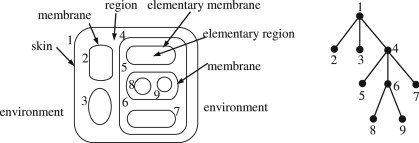
\includegraphics{img/membrane_structure.jpg}
  \caption{The membrane structure of a P system and its associated tree \cite{Zhang20101997AnalyzingRadarSignalsWithMembrane}}
  \label{fig:membrane_structure}
\end{figure}

% Membrane models

Recently, several computational models based on the membrane structure have been created.



% P systems

\subsubsection{P systems} % (fold)
\label{subs:p_systems}

P systems were introduced in 1998 as a system with membrane structure that contains multisets of objects and rewrite rules that are executed in a maximally parallel manner. Since then, a huge amount of variants have been created with various computation powers. We have investigated the power of several such variants. Additionally, we propose a new variant with a vacuum, where the rules can describe what will happen to an object that arrives to an empty membrane.

P systems with existing and newly proposed variants will be discussed in the chapter \ref{cha:p_systems}.

Aside from P systems, other models based on the membrane structure have been created such as the Calculus of Looping Sequences (CLS), which was inspired by P systems.

% subsubsection p_systems (end)


% CLS

\subsubsection{The Calculus of Looping Sequences} % (fold)
\label{subs:calculus_of_looping_sequences}

Barbuti in \cite{Barbuti07CLS} concluded that there is a need for a formalism having a simple notation, having the ability of describing biological systems at different levels of abstractions, having some notions of compositionality and being flexible enough to allow describing new kinds of phenomena as they are discovered, without being specialized to the description of a particular class of systems. The Calculus of Looping Sequences (CLS) was introduced in \cite{Barbuti07CLS}.

The membrane structure in CLS is defined recursively, consisting of terms $T$ and sequences $S$:
$$ T ::= S \mid (S)^L\rfloor T \mid T|T$$
$$ S ::= \eps \mid a \mid S\cdot S $$
, where $a$ is a symbol from the alphabet, $\eps$ represents the empty sequence, $\cdot$ is a sequencing operator, $(S)^L$ is a looping operator, $|$ is a parallel composition operator and $\rfloor$ is a containment operator.

Membranes are represented by a sequence that is looped around.
Several extensions of the CLS have been proposed. In CLS+ the looping operator can be applied to a parallel composition of sequences, which represents a notion of a fluid membrane.
CLS+ can be translated to CLS (see \cite{Barbuti07CLS}).
Milazzo in his PhD thesis \cite{Milazzo07CLS} includes also a simulation of a P system using CLS. The major difficulty is simulating the maximal parallelism of rule application.

% subsubsection calculus_of_looping_sequences (end)

% subsection membrane_systems (end)

% section biologically_inspired_computing_models (end)